


% Header, overrides base

    % Make sure that the sphinx doc style knows who it inherits from.
    \def\sphinxdocclass{article}

    % Declare the document class
    \documentclass[letterpaper,10pt,english]{/anaconda/lib/python2.7/site-packages/sphinx/texinputs/sphinxhowto}

    % Imports
    \usepackage[utf8]{inputenc}
    \DeclareUnicodeCharacter{00A0}{\\nobreakspace}
    \usepackage[T1]{fontenc}
    \usepackage{babel}
    \usepackage{times}
    \usepackage{import}
    \usepackage[Bjarne]{/anaconda/lib/python2.7/site-packages/sphinx/texinputs/fncychap}
    \usepackage{longtable}
    \usepackage{/anaconda/lib/python2.7/site-packages/sphinx/texinputs/sphinx}
    \usepackage{multirow}

    \usepackage{amsmath}
    \usepackage{amssymb}
    \usepackage{ucs}
    \usepackage{enumerate}

    % Used to make the Input/Output rules follow around the contents.
    \usepackage{needspace}

    % Pygments requirements
    \usepackage{fancyvrb}
    \usepackage{color}
    % ansi colors additions
    \definecolor{darkgreen}{rgb}{.12,.54,.11}
    \definecolor{lightgray}{gray}{.95}
    \definecolor{brown}{rgb}{0.54,0.27,0.07}
    \definecolor{purple}{rgb}{0.5,0.0,0.5}
    \definecolor{darkgray}{gray}{0.25}
    \definecolor{lightred}{rgb}{1.0,0.39,0.28}
    \definecolor{lightgreen}{rgb}{0.48,0.99,0.0}
    \definecolor{lightblue}{rgb}{0.53,0.81,0.92}
    \definecolor{lightpurple}{rgb}{0.87,0.63,0.87}
    \definecolor{lightcyan}{rgb}{0.5,1.0,0.83}

    % Needed to box output/input
    \usepackage{tikz}
        \usetikzlibrary{calc,arrows,shadows}
    \usepackage[framemethod=tikz]{mdframed}

    \usepackage{alltt}

    % Used to load and display graphics
    \usepackage{graphicx}
    \graphicspath{ {figs/} }
    \usepackage[Export]{adjustbox} % To resize

    % used so that images for notebooks which have spaces in the name can still be included
    \usepackage{grffile}


    % For formatting output while also word wrapping.
    \usepackage{listings}
    \lstset{breaklines=true}
    \lstset{basicstyle=\small\ttfamily}
    \def\smaller{\fontsize{9.5pt}{9.5pt}\selectfont}

    %Pygments definitions
    
\makeatletter
\def\PY@reset{\let\PY@it=\relax \let\PY@bf=\relax%
    \let\PY@ul=\relax \let\PY@tc=\relax%
    \let\PY@bc=\relax \let\PY@ff=\relax}
\def\PY@tok#1{\csname PY@tok@#1\endcsname}
\def\PY@toks#1+{\ifx\relax#1\empty\else%
    \PY@tok{#1}\expandafter\PY@toks\fi}
\def\PY@do#1{\PY@bc{\PY@tc{\PY@ul{%
    \PY@it{\PY@bf{\PY@ff{#1}}}}}}}
\def\PY#1#2{\PY@reset\PY@toks#1+\relax+\PY@do{#2}}

\expandafter\def\csname PY@tok@gd\endcsname{\def\PY@tc##1{\textcolor[rgb]{0.63,0.00,0.00}{##1}}}
\expandafter\def\csname PY@tok@gu\endcsname{\let\PY@bf=\textbf\def\PY@tc##1{\textcolor[rgb]{0.50,0.00,0.50}{##1}}}
\expandafter\def\csname PY@tok@gt\endcsname{\def\PY@tc##1{\textcolor[rgb]{0.00,0.27,0.87}{##1}}}
\expandafter\def\csname PY@tok@gs\endcsname{\let\PY@bf=\textbf}
\expandafter\def\csname PY@tok@gr\endcsname{\def\PY@tc##1{\textcolor[rgb]{1.00,0.00,0.00}{##1}}}
\expandafter\def\csname PY@tok@cm\endcsname{\let\PY@it=\textit\def\PY@tc##1{\textcolor[rgb]{0.25,0.50,0.50}{##1}}}
\expandafter\def\csname PY@tok@vg\endcsname{\def\PY@tc##1{\textcolor[rgb]{0.10,0.09,0.49}{##1}}}
\expandafter\def\csname PY@tok@m\endcsname{\def\PY@tc##1{\textcolor[rgb]{0.40,0.40,0.40}{##1}}}
\expandafter\def\csname PY@tok@mh\endcsname{\def\PY@tc##1{\textcolor[rgb]{0.40,0.40,0.40}{##1}}}
\expandafter\def\csname PY@tok@go\endcsname{\def\PY@tc##1{\textcolor[rgb]{0.53,0.53,0.53}{##1}}}
\expandafter\def\csname PY@tok@ge\endcsname{\let\PY@it=\textit}
\expandafter\def\csname PY@tok@vc\endcsname{\def\PY@tc##1{\textcolor[rgb]{0.10,0.09,0.49}{##1}}}
\expandafter\def\csname PY@tok@il\endcsname{\def\PY@tc##1{\textcolor[rgb]{0.40,0.40,0.40}{##1}}}
\expandafter\def\csname PY@tok@cs\endcsname{\let\PY@it=\textit\def\PY@tc##1{\textcolor[rgb]{0.25,0.50,0.50}{##1}}}
\expandafter\def\csname PY@tok@cp\endcsname{\def\PY@tc##1{\textcolor[rgb]{0.74,0.48,0.00}{##1}}}
\expandafter\def\csname PY@tok@gi\endcsname{\def\PY@tc##1{\textcolor[rgb]{0.00,0.63,0.00}{##1}}}
\expandafter\def\csname PY@tok@gh\endcsname{\let\PY@bf=\textbf\def\PY@tc##1{\textcolor[rgb]{0.00,0.00,0.50}{##1}}}
\expandafter\def\csname PY@tok@ni\endcsname{\let\PY@bf=\textbf\def\PY@tc##1{\textcolor[rgb]{0.60,0.60,0.60}{##1}}}
\expandafter\def\csname PY@tok@nl\endcsname{\def\PY@tc##1{\textcolor[rgb]{0.63,0.63,0.00}{##1}}}
\expandafter\def\csname PY@tok@nn\endcsname{\let\PY@bf=\textbf\def\PY@tc##1{\textcolor[rgb]{0.00,0.00,1.00}{##1}}}
\expandafter\def\csname PY@tok@no\endcsname{\def\PY@tc##1{\textcolor[rgb]{0.53,0.00,0.00}{##1}}}
\expandafter\def\csname PY@tok@na\endcsname{\def\PY@tc##1{\textcolor[rgb]{0.49,0.56,0.16}{##1}}}
\expandafter\def\csname PY@tok@nb\endcsname{\def\PY@tc##1{\textcolor[rgb]{0.00,0.50,0.00}{##1}}}
\expandafter\def\csname PY@tok@nc\endcsname{\let\PY@bf=\textbf\def\PY@tc##1{\textcolor[rgb]{0.00,0.00,1.00}{##1}}}
\expandafter\def\csname PY@tok@nd\endcsname{\def\PY@tc##1{\textcolor[rgb]{0.67,0.13,1.00}{##1}}}
\expandafter\def\csname PY@tok@ne\endcsname{\let\PY@bf=\textbf\def\PY@tc##1{\textcolor[rgb]{0.82,0.25,0.23}{##1}}}
\expandafter\def\csname PY@tok@nf\endcsname{\def\PY@tc##1{\textcolor[rgb]{0.00,0.00,1.00}{##1}}}
\expandafter\def\csname PY@tok@si\endcsname{\let\PY@bf=\textbf\def\PY@tc##1{\textcolor[rgb]{0.73,0.40,0.53}{##1}}}
\expandafter\def\csname PY@tok@s2\endcsname{\def\PY@tc##1{\textcolor[rgb]{0.73,0.13,0.13}{##1}}}
\expandafter\def\csname PY@tok@vi\endcsname{\def\PY@tc##1{\textcolor[rgb]{0.10,0.09,0.49}{##1}}}
\expandafter\def\csname PY@tok@nt\endcsname{\let\PY@bf=\textbf\def\PY@tc##1{\textcolor[rgb]{0.00,0.50,0.00}{##1}}}
\expandafter\def\csname PY@tok@nv\endcsname{\def\PY@tc##1{\textcolor[rgb]{0.10,0.09,0.49}{##1}}}
\expandafter\def\csname PY@tok@s1\endcsname{\def\PY@tc##1{\textcolor[rgb]{0.73,0.13,0.13}{##1}}}
\expandafter\def\csname PY@tok@sh\endcsname{\def\PY@tc##1{\textcolor[rgb]{0.73,0.13,0.13}{##1}}}
\expandafter\def\csname PY@tok@sc\endcsname{\def\PY@tc##1{\textcolor[rgb]{0.73,0.13,0.13}{##1}}}
\expandafter\def\csname PY@tok@sx\endcsname{\def\PY@tc##1{\textcolor[rgb]{0.00,0.50,0.00}{##1}}}
\expandafter\def\csname PY@tok@bp\endcsname{\def\PY@tc##1{\textcolor[rgb]{0.00,0.50,0.00}{##1}}}
\expandafter\def\csname PY@tok@c1\endcsname{\let\PY@it=\textit\def\PY@tc##1{\textcolor[rgb]{0.25,0.50,0.50}{##1}}}
\expandafter\def\csname PY@tok@kc\endcsname{\let\PY@bf=\textbf\def\PY@tc##1{\textcolor[rgb]{0.00,0.50,0.00}{##1}}}
\expandafter\def\csname PY@tok@c\endcsname{\let\PY@it=\textit\def\PY@tc##1{\textcolor[rgb]{0.25,0.50,0.50}{##1}}}
\expandafter\def\csname PY@tok@mf\endcsname{\def\PY@tc##1{\textcolor[rgb]{0.40,0.40,0.40}{##1}}}
\expandafter\def\csname PY@tok@err\endcsname{\def\PY@bc##1{\setlength{\fboxsep}{0pt}\fcolorbox[rgb]{1.00,0.00,0.00}{1,1,1}{\strut ##1}}}
\expandafter\def\csname PY@tok@kd\endcsname{\let\PY@bf=\textbf\def\PY@tc##1{\textcolor[rgb]{0.00,0.50,0.00}{##1}}}
\expandafter\def\csname PY@tok@ss\endcsname{\def\PY@tc##1{\textcolor[rgb]{0.10,0.09,0.49}{##1}}}
\expandafter\def\csname PY@tok@sr\endcsname{\def\PY@tc##1{\textcolor[rgb]{0.73,0.40,0.53}{##1}}}
\expandafter\def\csname PY@tok@mo\endcsname{\def\PY@tc##1{\textcolor[rgb]{0.40,0.40,0.40}{##1}}}
\expandafter\def\csname PY@tok@kn\endcsname{\let\PY@bf=\textbf\def\PY@tc##1{\textcolor[rgb]{0.00,0.50,0.00}{##1}}}
\expandafter\def\csname PY@tok@mi\endcsname{\def\PY@tc##1{\textcolor[rgb]{0.40,0.40,0.40}{##1}}}
\expandafter\def\csname PY@tok@gp\endcsname{\let\PY@bf=\textbf\def\PY@tc##1{\textcolor[rgb]{0.00,0.00,0.50}{##1}}}
\expandafter\def\csname PY@tok@o\endcsname{\def\PY@tc##1{\textcolor[rgb]{0.40,0.40,0.40}{##1}}}
\expandafter\def\csname PY@tok@kr\endcsname{\let\PY@bf=\textbf\def\PY@tc##1{\textcolor[rgb]{0.00,0.50,0.00}{##1}}}
\expandafter\def\csname PY@tok@s\endcsname{\def\PY@tc##1{\textcolor[rgb]{0.73,0.13,0.13}{##1}}}
\expandafter\def\csname PY@tok@kp\endcsname{\def\PY@tc##1{\textcolor[rgb]{0.00,0.50,0.00}{##1}}}
\expandafter\def\csname PY@tok@w\endcsname{\def\PY@tc##1{\textcolor[rgb]{0.73,0.73,0.73}{##1}}}
\expandafter\def\csname PY@tok@kt\endcsname{\def\PY@tc##1{\textcolor[rgb]{0.69,0.00,0.25}{##1}}}
\expandafter\def\csname PY@tok@ow\endcsname{\let\PY@bf=\textbf\def\PY@tc##1{\textcolor[rgb]{0.67,0.13,1.00}{##1}}}
\expandafter\def\csname PY@tok@sb\endcsname{\def\PY@tc##1{\textcolor[rgb]{0.73,0.13,0.13}{##1}}}
\expandafter\def\csname PY@tok@k\endcsname{\let\PY@bf=\textbf\def\PY@tc##1{\textcolor[rgb]{0.00,0.50,0.00}{##1}}}
\expandafter\def\csname PY@tok@se\endcsname{\let\PY@bf=\textbf\def\PY@tc##1{\textcolor[rgb]{0.73,0.40,0.13}{##1}}}
\expandafter\def\csname PY@tok@sd\endcsname{\let\PY@it=\textit\def\PY@tc##1{\textcolor[rgb]{0.73,0.13,0.13}{##1}}}

\def\PYZbs{\char`\\}
\def\PYZus{\char`\_}
\def\PYZob{\char`\{}
\def\PYZcb{\char`\}}
\def\PYZca{\char`\^}
\def\PYZam{\char`\&}
\def\PYZlt{\char`\<}
\def\PYZgt{\char`\>}
\def\PYZsh{\char`\#}
\def\PYZpc{\char`\%}
\def\PYZdl{\char`\$}
\def\PYZhy{\char`\-}
\def\PYZsq{\char`\'}
\def\PYZdq{\char`\"}
\def\PYZti{\char`\~}
% for compatibility with earlier versions
\def\PYZat{@}
\def\PYZlb{[}
\def\PYZrb{]}
\makeatother


    %Set pygments styles if needed...
    
        \definecolor{nbframe-border}{rgb}{0.867,0.867,0.867}
        \definecolor{nbframe-bg}{rgb}{0.969,0.969,0.969}
        \definecolor{nbframe-in-prompt}{rgb}{0.0,0.0,0.502}
        \definecolor{nbframe-out-prompt}{rgb}{0.545,0.0,0.0}

        \newenvironment{ColorVerbatim}
        {\begin{mdframed}[%
            roundcorner=1.0pt, %
            backgroundcolor=nbframe-bg, %
            userdefinedwidth=1\linewidth, %
            leftmargin=0.1\linewidth, %
            innerleftmargin=0pt, %
            innerrightmargin=0pt, %
            linecolor=nbframe-border, %
            linewidth=1pt, %
            usetwoside=false, %
            everyline=true, %
            innerlinewidth=3pt, %
            innerlinecolor=nbframe-bg, %
            middlelinewidth=1pt, %
            middlelinecolor=nbframe-bg, %
            outerlinewidth=0.5pt, %
            outerlinecolor=nbframe-border, %
            needspace=0pt
        ]}
        {\end{mdframed}}
        
        \newenvironment{InvisibleVerbatim}
        {\begin{mdframed}[leftmargin=0.1\linewidth,innerleftmargin=3pt,innerrightmargin=3pt, userdefinedwidth=1\linewidth, linewidth=0pt, linecolor=white, usetwoside=false]}
        {\end{mdframed}}

        \renewenvironment{Verbatim}[1][\unskip]
        {\begin{alltt}\smaller}
        {\end{alltt}}
    

    % Help prevent overflowing lines due to urls and other hard-to-break 
    % entities.  This doesn't catch everything...
    \sloppy

    % Document level variables
    \title{NFL-Go-For-It!}
    \date{April 24, 2014}
    \release{}
    \author{Unknown Author}
    \renewcommand{\releasename}{}

    % TODO: Add option for the user to specify a logo for his/her export.
    \newcommand{\sphinxlogo}{}

    % Make the index page of the document.
    \makeindex

    % Import sphinx document type specifics.
     


% Body

    % Start of the document
    \begin{document}

        
            \maketitle
        

        


        
        NFL Go For It! \textbackslash{}by Mike Ghirardo and Thomas McCann \textbackslash{}In football there are many decisions a team needs to make in order win
the game. In this project we focus on the decision that needs to be made
on the 4th down of any given play. There are three decisions to be made
on the fourth down. 1. Punt the ball 2. Kick a field goal 3. Go for a
first down In this project we try to determine which decision should be
made under certain conditions. The following are the conditions which we
take into account in determining the decision. 1. Offensive and
defensive rank of the offensive team. 2. Offensive and defensive rank of
the defensive team. 3. The number of yards to convert for a first down.
4. The field position started from. With this information from the data
we were able to estimate the expected points scored for each of the of
three decisions. Finally, with this information a decision can be made.

    

        % If the first block is an image, minipage the image.  Else
        % request a certain amount of space for the input text.
        \needspace{4\baselineskip}
        
        

            % Add document contents.
            
                \begin{InvisibleVerbatim}
                \vspace{-0.5\baselineskip}
\begin{alltt}Populating the interactive namespace from numpy and matplotlib
\end{alltt}

            \end{InvisibleVerbatim}
            
        
    
Importing NFL play-by-play data from years 2002 to 2012.

    

        % If the first block is an image, minipage the image.  Else
        % request a certain amount of space for the input text.
        \needspace{4\baselineskip}
        
        

            % Add document contents.
            
                \makebox[0.1\linewidth]{\smaller\hfill\tt\color{nbframe-out-prompt}Out\hspace{4pt}{[}2{]}:\hspace{4pt}}\\*
                \vspace{-2.55\baselineskip}\begin{InvisibleVerbatim}
                \vspace{-0.5\baselineskip}
\begin{alltt}0\end{alltt}

            \end{InvisibleVerbatim}
            
        
    
Joining data sets together to get one long dataset of play-by-play data
accross all 11 years.
Taking out post-season games to get a more accurate ranking of teams.
The following retrieves the first and last plays of each game. This will
be useful in helping us determine team ranks by how many points scored
per game and how many points let go per game.
The following sums points gained and points let go per game per team per
season. The means by which the teams are ranked offensively and
defensively is taking the total number of points scored and total number
of points let go and adding them.
Creating a two matrices of the total points scored and total points let
go with the season as the column and the team as the row, and then
ranking them to get the offensive and defensive ranks.
Here we bring in the team rankings into the main data frame.
Here we create dummy variables and factor variables concerning the
ranking of teams. This will help us run a logistic regression using team
ranking as covariates.


The following gives drive by drive information. This information is
useful in helping us know the expected number of points the offensive
team will score given they started the first play of the drive on a
specific yard line.
The following code quantifies the consequences of certain events
occurring. We create a vector of the number of points scored at the end
of a teams drive. We assume that touchdown plays automatically get seven
points, which means we assume the team gets the extra point given they
score a touchdown. Then we run a multinomial logistic regression to
determine the likelihood of these events based on certain factors, such
as team rank and field position. With both pieces of information we
determine the expected number points of a team given they convert a
first down, their ranking and their field position.

    

        % If the first block is an image, minipage the image.  Else
        % request a certain amount of space for the input text.
        \needspace{4\baselineskip}
        
        

            % Add document contents.
            
                \begin{InvisibleVerbatim}
                \vspace{-0.5\baselineskip}
\begin{alltt}Optimization terminated successfully.
         Current function value: 0.872453
         Iterations 12
\end{alltt}

            \end{InvisibleVerbatim}
            
                \makebox[0.1\linewidth]{\smaller\hfill\tt\color{nbframe-out-prompt}Out\hspace{4pt}{[}12{]}:\hspace{4pt}}\\*
                \vspace{-2.55\baselineskip}\begin{InvisibleVerbatim}
                \vspace{-0.5\baselineskip}
\begin{alltt}<class 'statsmodels.iolib.summary.Summary'>
"""
                          MNLogit Regression Results
======================================================================
========
Dep. Variable:                  score   No. Observations:
65105
Model:                        MNLogit   Df Residuals:
65081
Method:                           MLE   Df Model:
20
Date:                Thu, 24 Apr 2014   Pseudo R-squ.:
0.05169
Time:                        23:01:18   Log-Likelihood:
-56801.
converged:                       True   LL-Null:
-59897.
                                        LLR p-value:
0.000
======================================================================
==========
   score=DefTD       coef    std err          z      P>|z|      [95.0\%
Conf. Int.]
----------------------------------------------------------------------
------------
intercept         17.1021      1.159     14.759      0.000
14.831    19.373
ydline            -0.1892      0.012    -15.208      0.000
-0.214    -0.165
offrankMid         0.0065      0.010      0.620      0.535
-0.014     0.027
offrank31t32       0.0238      0.347      0.069      0.945
-0.656     0.704
defrankMid         0.0103      0.010      1.018      0.309
-0.010     0.030
defrank31t32       0.4581      0.395      1.161      0.246
-0.315     1.231
----------------------------------------------------------------------
------------
    score=FG       coef    std err          z      P>|z|      [95.0\%
Conf. Int.]
----------------------------------------------------------------------
----------
intercept       23.3837      1.125     20.785      0.000        21.179
25.589
ydline          -0.2381      0.012    -19.834      0.000        -0.262
-0.215
offrankMid      -0.0052      0.009     -0.565      0.572        -0.023
0.013
offrank31t32    -0.7413      0.308     -2.410      0.016        -1.344
-0.139
defrankMid       0.0217      0.009      2.428      0.015         0.004
0.039
defrank31t32     0.3214      0.357      0.901      0.368        -0.378
1.021
----------------------------------------------------------------------
----------
score=NoPoints       coef    std err          z      P>|z|      [95.0\%
Conf. Int.]
----------------------------------------------------------------------
------------
intercept         22.7030      1.124     20.200      0.000
20.500    24.906
ydline            -0.2050      0.012    -17.097      0.000
-0.228    -0.181
offrankMid         0.0080      0.009      0.870      0.384
-0.010     0.026
offrank31t32      -0.2494      0.303     -0.823      0.411
-0.844     0.345
defrankMid         0.0104      0.009      1.174      0.241
-0.007     0.028
defrank31t32       0.0488      0.354      0.138      0.890
-0.644     0.742
----------------------------------------------------------------------
------------
    score=TD       coef    std err          z      P>|z|      [95.0\%
Conf. Int.]
----------------------------------------------------------------------
----------
intercept       23.6977      1.125     21.070      0.000        21.493
25.902
ydline          -0.2343      0.012    -19.524      0.000        -0.258
-0.211
offrankMid      -0.0209      0.009     -2.270      0.023        -0.039
-0.003
offrank31t32    -1.3770      0.307     -4.487      0.000        -1.979
-0.775
defrankMid       0.0302      0.009      3.393      0.001         0.013
0.048
defrank31t32     0.7186      0.355      2.023      0.043         0.023
1.415
======================================================================
==========
"""\end{alltt}

            \end{InvisibleVerbatim}
            
        
    


    

        % If the first block is an image, minipage the image.  Else
        % request a certain amount of space for the input text.
        \needspace{4\baselineskip}
        
        

            % Add document contents.
            
                \makebox[0.1\linewidth]{\smaller\hfill\tt\color{nbframe-out-prompt}Out\hspace{4pt}{[}13{]}:\hspace{4pt}}\\*
                \vspace{-2.55\baselineskip}\begin{InvisibleVerbatim}
                \vspace{-0.5\baselineskip}
\begin{alltt}                  DefTD         FG   NoPoints         TD
intercept     17.102051  23.383689  22.702956  23.697687
ydline        -0.189247  -0.238087  -0.204967  -0.234290
offrankMid     0.006484  -0.005221   0.007977  -0.020917
offrank31t32   0.023844  -0.741291  -0.249409  -1.376970
defrankMid     0.010301   0.021678   0.010377   0.030189
defrank31t32   0.458122   0.321432   0.048783   0.718639

[6 rows x 4 columns]\end{alltt}

            \end{InvisibleVerbatim}
            
        
    
The following is code concerning the decision to punt. Here, we find all
punt plays and using logistic regression we determine the probability of
events happening given that the team making the decision punted the ball
at a certain yard line. The other team receiveing the punt can then
score an offensive touchdown or field goal, get no points or give up a
defensive touchdown or safety.

    

        % If the first block is an image, minipage the image.  Else
        % request a certain amount of space for the input text.
        \needspace{4\baselineskip}
        
        

            % Add document contents.
            
                \begin{InvisibleVerbatim}
                \vspace{-0.5\baselineskip}
\begin{alltt}Optimization terminated successfully.
         Current function value: 0.881161
         Iterations 9
\end{alltt}

            \end{InvisibleVerbatim}
            
                \makebox[0.1\linewidth]{\smaller\hfill\tt\color{nbframe-out-prompt}Out\hspace{4pt}{[}14{]}:\hspace{4pt}}\\*
                \vspace{-2.55\baselineskip}\begin{InvisibleVerbatim}
                \vspace{-0.5\baselineskip}
\begin{alltt}<class 'statsmodels.iolib.summary.Summary'>
"""
                          MNLogit Regression Results
======================================================================
========
Dep. Variable:                  score   No. Observations:
26271
Model:                        MNLogit   Df Residuals:
26247
Method:                           MLE   Df Model:
20
Date:                Thu, 24 Apr 2014   Pseudo R-squ.:
0.03018
Time:                        23:01:21   Log-Likelihood:
-23149.
converged:                       True   LL-Null:
-23869.
                                        LLR p-value:
2.247e-293
======================================================================
===============
      score=DefTD       coef    std err          z      P>|z|
[95.0\% Conf. Int.]
----------------------------------------------------------------------
---------------
intercept            -2.5052      0.567     -4.415      0.000
-3.617    -1.393
removelast\_ydline     0.0502      0.009      5.741      0.000
0.033     0.067
offrankMid            0.0073      0.014      0.520      0.603
-0.020     0.035
offrank31t32         -0.1668      0.431     -0.387      0.699
-1.011     0.678
defrankMid            0.0189      0.013      1.431      0.153
-0.007     0.045
defrank31t32          0.2559      0.592      0.432      0.666
-0.905     1.417
----------------------------------------------------------------------
---------------
         score=FG       coef    std err          z      P>|z|
[95.0\% Conf. Int.]
----------------------------------------------------------------------
---------------
intercept            -2.0875      0.461     -4.532      0.000
-2.990    -1.185
removelast\_ydline     0.0874      0.007     11.719      0.000
0.073     0.102
offrankMid           -0.0018      0.012     -0.154      0.878
-0.024     0.021
offrank31t32         -0.9428      0.348     -2.712      0.007
-1.624    -0.262
defrankMid            0.0284      0.011      2.621      0.009
0.007     0.050
defrank31t32          0.6024      0.488      1.235      0.217
-0.354     1.558
----------------------------------------------------------------------
---------------
   score=NoPoints       coef    std err          z      P>|z|
[95.0\% Conf. Int.]
----------------------------------------------------------------------
---------------
intercept             1.3069      0.451      2.897      0.004
0.423     2.191
removelast\_ydline     0.0607      0.007      8.239      0.000
0.046     0.075
offrankMid            0.0132      0.011      1.160      0.246
-0.009     0.036
offrank31t32         -0.3978      0.338     -1.176      0.240
-1.061     0.265
defrankMid            0.0149      0.011      1.395      0.163
-0.006     0.036
defrank31t32          0.2583      0.482      0.536      0.592
-0.687     1.204
----------------------------------------------------------------------
---------------
         score=TD       coef    std err          z      P>|z|
[95.0\% Conf. Int.]
----------------------------------------------------------------------
---------------
intercept            -1.1274      0.457     -2.469      0.014
-2.022    -0.233
removelast\_ydline     0.0802      0.007     10.814      0.000
0.066     0.095
offrankMid           -0.0164      0.011     -1.428      0.153
-0.039     0.006
offrank31t32         -1.4860      0.346     -4.295      0.000
-2.164    -0.808
defrankMid            0.0381      0.011      3.529      0.000
0.017     0.059
defrank31t32          1.1201      0.485      2.311      0.021
0.170     2.070
======================================================================
===============
"""\end{alltt}

            \end{InvisibleVerbatim}
            
        
    


    

        % If the first block is an image, minipage the image.  Else
        % request a certain amount of space for the input text.
        \needspace{4\baselineskip}
        
        

            % Add document contents.
            
                \makebox[0.1\linewidth]{\smaller\hfill\tt\color{nbframe-out-prompt}Out\hspace{4pt}{[}15{]}:\hspace{4pt}}\\*
                \vspace{-2.55\baselineskip}\begin{InvisibleVerbatim}
                \vspace{-0.5\baselineskip}
\begin{alltt}                      DefTD        FG  NoPoints        TD
intercept         -2.505152 -2.087459  1.306882 -1.127434
removelast\_ydline  0.050217  0.087383  0.060661  0.080226
offrankMid         0.007299 -0.001777  0.013215 -0.016401
offrank31t32      -0.166807 -0.942778 -0.397772 -1.485986
defrankMid         0.018914  0.028430  0.014893  0.038073
defrank31t32       0.255890  0.602383  0.258313  1.120144

[6 rows x 4 columns]\end{alltt}

            \end{InvisibleVerbatim}
            
        
    
The following code is used to pull out fourth down plays from the data.
This is important since we'll use plays from these downs to find the
expected number of points given field goal attempt, punt attempt, or go
for it attempt.
Pulling out field goal attempt data and running a logistic regression to
determine the likelihood of converting depending on the yardline the
field goal is attempted from.

    

        % If the first block is an image, minipage the image.  Else
        % request a certain amount of space for the input text.
        \needspace{4\baselineskip}
        
        

            % Add document contents.
            
                \begin{InvisibleVerbatim}
                \vspace{-0.5\baselineskip}
\begin{alltt}Optimization terminated successfully.
         Current function value: 0.410096
         Iterations 7
\end{alltt}

            \end{InvisibleVerbatim}
            
                \makebox[0.1\linewidth]{\smaller\hfill\tt\color{nbframe-out-prompt}Out\hspace{4pt}{[}17{]}:\hspace{4pt}}\\*
                \vspace{-2.55\baselineskip}\begin{InvisibleVerbatim}
                \vspace{-0.5\baselineskip}
\begin{alltt}<class 'statsmodels.iolib.summary.Summary'>
"""
                           Logit Regression Results
======================================================================
========
Dep. Variable:              converted   No. Observations:
9650
Model:                          Logit   Df Residuals:
9648
Method:                           MLE   Df Model:
1
Date:                Thu, 24 Apr 2014   Pseudo R-squ.:
0.1206
Time:                        23:01:21   Log-Likelihood:
-3957.4
converged:                       True   LL-Null:
-4500.1
                                        LLR p-value:
5.246e-238
======================================================================
========
                 coef    std err          z      P>|z|      [95.0\%
Conf. Int.]
----------------------------------------------------------------------
--------
intercept      3.6030      0.083     43.532      0.000         3.441
3.765
ydline        -0.0981      0.003    -29.699      0.000        -0.105
-0.092
======================================================================
========
"""\end{alltt}

            \end{InvisibleVerbatim}
            
        
    

The following pulls out the rankings of teams and yards to go to convert
on the fourth down. We also perform a logistic regression to determine
the likelihood of converting given the rankings and yards to go.

    

        % If the first block is an image, minipage the image.  Else
        % request a certain amount of space for the input text.
        \needspace{4\baselineskip}
        
        

            % Add document contents.
            
                \begin{InvisibleVerbatim}
                \vspace{-0.5\baselineskip}
\begin{alltt}Optimization terminated successfully.
         Current function value: 0.653088
         Iterations 5
\end{alltt}

            \end{InvisibleVerbatim}
            
                \makebox[0.1\linewidth]{\smaller\hfill\tt\color{nbframe-out-prompt}Out\hspace{4pt}{[}19{]}:\hspace{4pt}}\\*
                \vspace{-2.55\baselineskip}\begin{InvisibleVerbatim}
                \vspace{-0.5\baselineskip}
\begin{alltt}<class 'statsmodels.iolib.summary.Summary'>
"""
                           Logit Regression Results
======================================================================
========
Dep. Variable:              converted   No. Observations:
5494
Model:                          Logit   Df Residuals:
5488
Method:                           MLE   Df Model:
5
Date:                Thu, 24 Apr 2014   Pseudo R-squ.:
0.05691
Time:                        23:01:22   Log-Likelihood:
-3588.1
converged:                       True   LL-Null:
-3804.6
                                        LLR p-value:
2.247e-91
======================================================================
==========
                   coef    std err          z      P>|z|      [95.0\%
Conf. Int.]
----------------------------------------------------------------------
----------
intercept        0.5808      0.082      7.067      0.000         0.420
0.742
togo            -0.1199      0.007    -17.664      0.000        -0.133
-0.107
offrankMid      -0.0076      0.003     -2.358      0.018        -0.014
-0.001
offrank31t32    -0.4553      0.122     -3.730      0.000        -0.695
-0.216
defrankMid       0.0112      0.003      3.510      0.000         0.005
0.017
defrank31t32     0.4841      0.135      3.578      0.000         0.219
0.749
======================================================================
==========
"""\end{alltt}

            \end{InvisibleVerbatim}
            
        
    

The following functions will be used to determine the choice to be made
given yard line, yards to go, and both offensive and defensive rankings
of the team making the decision as well as the other team.







convert\_prob is a three dimensional matrix that gives the probability
of the offensive team converting a first down given how many yards to go
for the first down, the offensive rank of the offense and the defensive
rank of the defense.

The following is a plot of total points scored on offense per season per
ranked team. Each color represents a different rank.

    

        % If the first block is an image, minipage the image.  Else
        % request a certain amount of space for the input text.
        \needspace{4\baselineskip}
        
        

            % Add document contents.
            
                \begin{InvisibleVerbatim}
                \vspace{-0.5\baselineskip}
    \begin{center}
    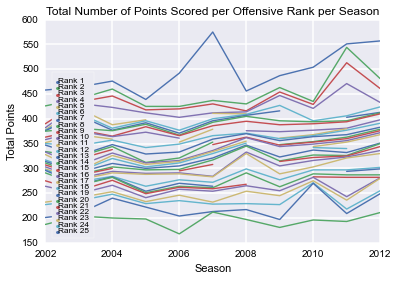
\includegraphics[max size={\textwidth}{\textheight}]{NFL-Go-For-It!_files/NFL-Go-For-It!_51_0.png}
    \par
    \end{center}
    
            \end{InvisibleVerbatim}
            
        
    
The following is a plot of total points scored on a defense per season
per ranked team. Each color represents a different rank.

    

        % If the first block is an image, minipage the image.  Else
        % request a certain amount of space for the input text.
        \needspace{4\baselineskip}
        
        

            % Add document contents.
            
                \begin{InvisibleVerbatim}
                \vspace{-0.5\baselineskip}
    \begin{center}
    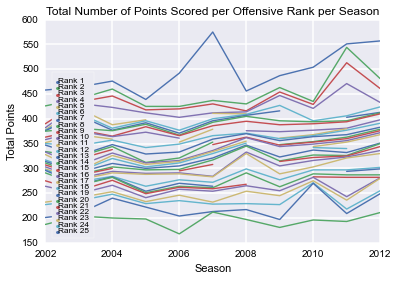
\includegraphics[max size={\textwidth}{\textheight}]{NFL-Go-For-It!_files/NFL-Go-For-It!_53_0.png}
    \par
    \end{center}
    
            \end{InvisibleVerbatim}
            
        
    
The following graph has probabilities of converting field goals on the
y-axis and the yardline the field goal is attempted from. In the midterm
presentation the shading on the following graph was purely aesthetic.
After creating vectors of the standard errors the following graph now
contains the actual confidence interval.

    

        % If the first block is an image, minipage the image.  Else
        % request a certain amount of space for the input text.
        \needspace{4\baselineskip}
        
        

            % Add document contents.
            
                \begin{InvisibleVerbatim}
                \vspace{-0.5\baselineskip}
    \begin{center}
    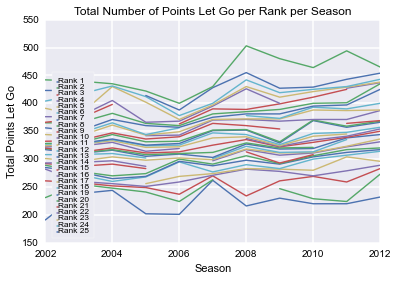
\includegraphics[max size={\textwidth}{\textheight}]{NFL-Go-For-It!_files/NFL-Go-For-It!_55_0.png}
    \par
    \end{center}
    
            \end{InvisibleVerbatim}
            
        
    
The following is the plot of the decision that should be made from the
30 yard line, where the offensive team has an outstanding ranking and
the defensive team is ranked poorly.

    

        % If the first block is an image, minipage the image.  Else
        % request a certain amount of space for the input text.
        \needspace{4\baselineskip}
        
        

            % Add document contents.
            
                \begin{InvisibleVerbatim}
                \vspace{-0.5\baselineskip}
    \begin{center}
    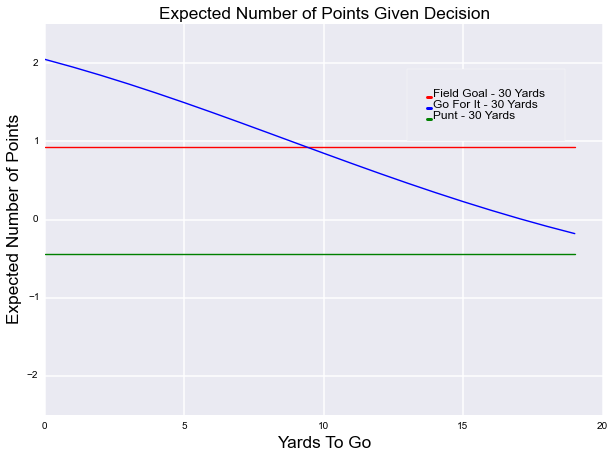
\includegraphics[max size={\textwidth}{\textheight}]{NFL-Go-For-It!_files/NFL-Go-For-It!_57_0.png}
    \par
    \end{center}
    
            \end{InvisibleVerbatim}
            
        
    
The following is the plot of the decision that should be made from the
30 yard line, where the offensive team has an mediocre ranking and the
defensive team is ranked mediocre.

    

        % If the first block is an image, minipage the image.  Else
        % request a certain amount of space for the input text.
        \needspace{4\baselineskip}
        
        

            % Add document contents.
            
                \begin{InvisibleVerbatim}
                \vspace{-0.5\baselineskip}
    \begin{center}
    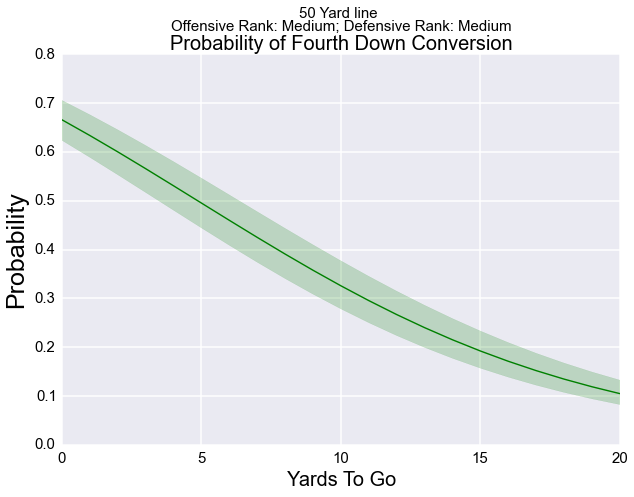
\includegraphics[max size={\textwidth}{\textheight}]{NFL-Go-For-It!_files/NFL-Go-For-It!_59_0.png}
    \par
    \end{center}
    
            \end{InvisibleVerbatim}
            
        
    
The following is the plot of the decision that should be made from the
30 yard line, where the offensive team has a poor ranking and the
defensive team is ranked highly.

    

        % If the first block is an image, minipage the image.  Else
        % request a certain amount of space for the input text.
        \needspace{4\baselineskip}
        
        

            % Add document contents.
            
                \begin{InvisibleVerbatim}
                \vspace{-0.5\baselineskip}
    \begin{center}
    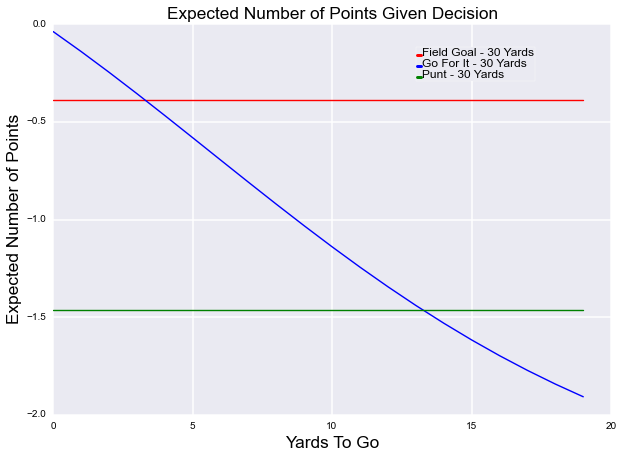
\includegraphics[max size={\textwidth}{\textheight}]{NFL-Go-For-It!_files/NFL-Go-For-It!_61_0.png}
    \par
    \end{center}
    
            \end{InvisibleVerbatim}
            
        
    

The following gives the decision to be made given high ranking of the
offensive team and poor ranking of the defensive team.


    

        % If the first block is an image, minipage the image.  Else
        % request a certain amount of space for the input text.
        \needspace{4\baselineskip}
        
        

            % Add document contents.
            
                \begin{InvisibleVerbatim}
                \vspace{-0.5\baselineskip}
    \begin{center}
    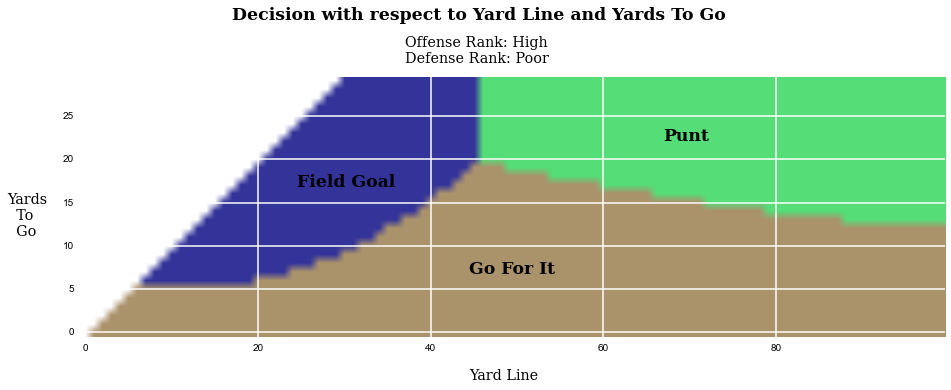
\includegraphics[max size={\textwidth}{\textheight}]{NFL-Go-For-It!_files/NFL-Go-For-It!_65_0.png}
    \par
    \end{center}
    
            \end{InvisibleVerbatim}
            
        
    
The following gives the decision to be made given mediocre ranking of
the offensive team and mediocre ranking of the defensive team.


    

        % If the first block is an image, minipage the image.  Else
        % request a certain amount of space for the input text.
        \needspace{4\baselineskip}
        
        

            % Add document contents.
            
                \begin{InvisibleVerbatim}
                \vspace{-0.5\baselineskip}
    \begin{center}
    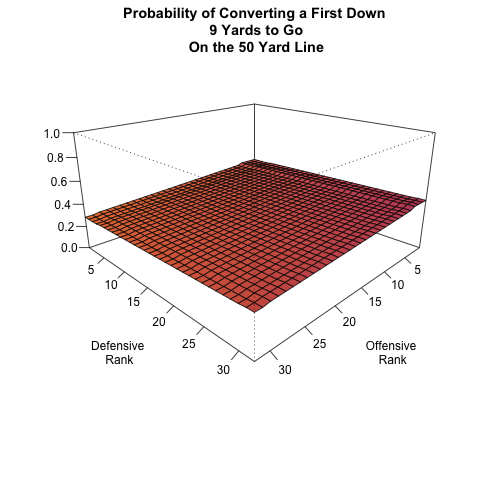
\includegraphics[max size={\textwidth}{\textheight}]{NFL-Go-For-It!_files/NFL-Go-For-It!_68_0.png}
    \par
    \end{center}
    
            \end{InvisibleVerbatim}
            
        
    
The following gives the decision to be made given poor ranking of the
offensive team and high ranking of the defensive team.


    

        % If the first block is an image, minipage the image.  Else
        % request a certain amount of space for the input text.
        \needspace{4\baselineskip}
        
        

            % Add document contents.
            
                \begin{InvisibleVerbatim}
                \vspace{-0.5\baselineskip}
    \begin{center}
    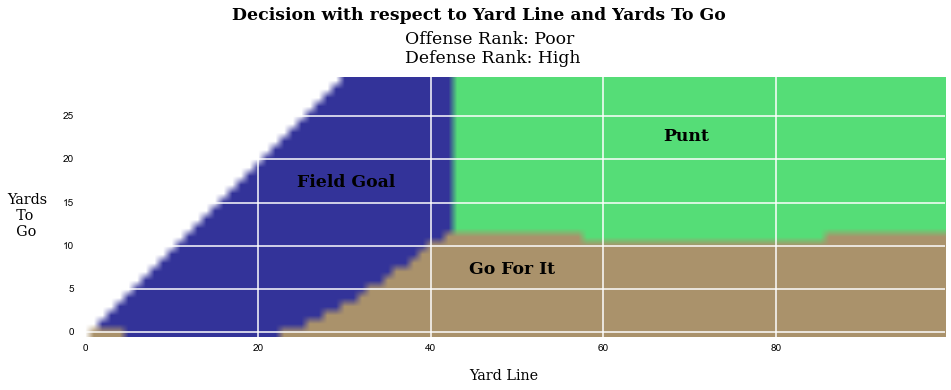
\includegraphics[max size={\textwidth}{\textheight}]{NFL-Go-For-It!_files/NFL-Go-For-It!_71_0.png}
    \par
    \end{center}
    
            \end{InvisibleVerbatim}
            
        
    
The following shows the probability of conversion of first down per
offensive and defensive rankings with 1 yard to go.

    

        % If the first block is an image, minipage the image.  Else
        % request a certain amount of space for the input text.
        \needspace{4\baselineskip}
        
        

            % Add document contents.
            
                \begin{InvisibleVerbatim}
                \vspace{-0.5\baselineskip}
    \begin{center}
    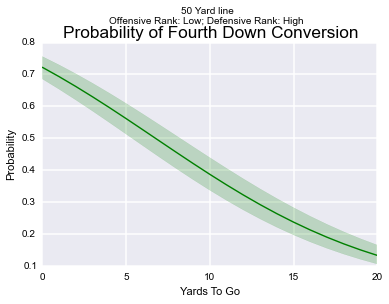
\includegraphics[max size={\textwidth}{\textheight}]{NFL-Go-For-It!_files/NFL-Go-For-It!_73_0.png}
    \par
    \end{center}
    
            \end{InvisibleVerbatim}
            
        
    
The following shows the probability of conversion of first down per
offensive and defensive rankings with 3 yard to go.

    

        % If the first block is an image, minipage the image.  Else
        % request a certain amount of space for the input text.
        \needspace{4\baselineskip}
        
        

            % Add document contents.
            
                \begin{InvisibleVerbatim}
                \vspace{-0.5\baselineskip}
    \begin{center}
    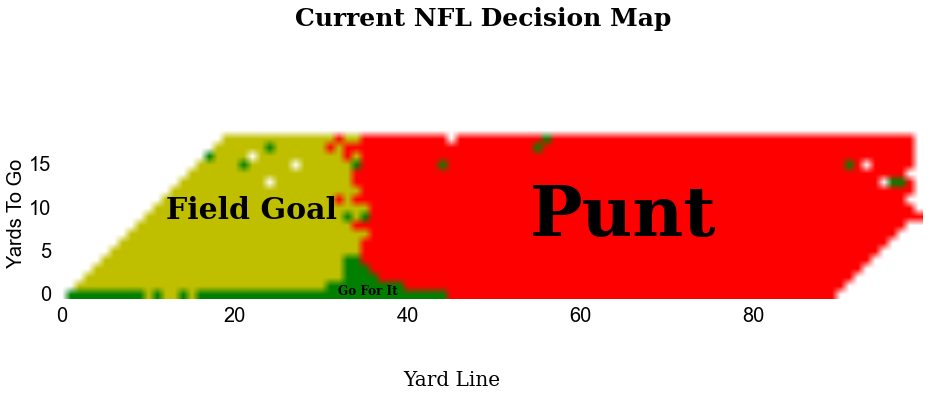
\includegraphics[max size={\textwidth}{\textheight}]{NFL-Go-For-It!_files/NFL-Go-For-It!_75_0.png}
    \par
    \end{center}
    
            \end{InvisibleVerbatim}
            
        
    
The following shows the probability of conversion of firt down per
offensive and defensive rankings with 6 yard to go.

    

        % If the first block is an image, minipage the image.  Else
        % request a certain amount of space for the input text.
        \needspace{4\baselineskip}
        
        

            % Add document contents.
            
                \begin{InvisibleVerbatim}
                \vspace{-0.5\baselineskip}
    \begin{center}
    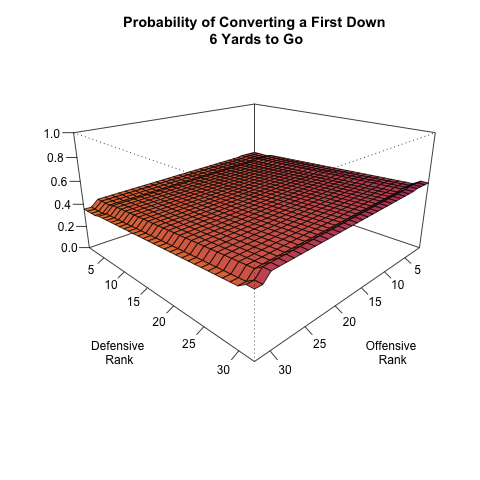
\includegraphics[max size={\textwidth}{\textheight}]{NFL-Go-For-It!_files/NFL-Go-For-It!_77_0.png}
    \par
    \end{center}
    
            \end{InvisibleVerbatim}
            
        
    
The following shows the probability of conversion of firt down per
offensive and defensive rankings with 9 yard to go.

    

        % If the first block is an image, minipage the image.  Else
        % request a certain amount of space for the input text.
        \needspace{4\baselineskip}
        
        

            % Add document contents.
            
                \begin{InvisibleVerbatim}
                \vspace{-0.5\baselineskip}
    \begin{center}
    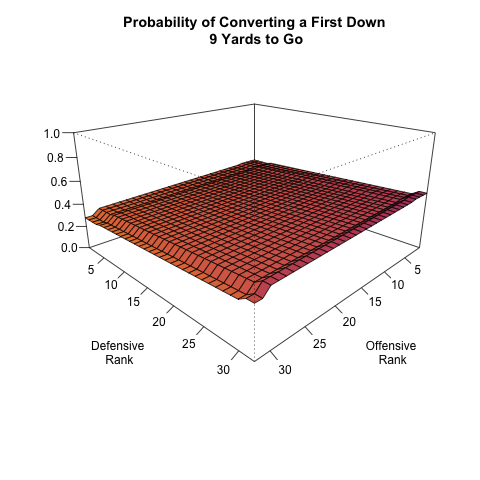
\includegraphics[max size={\textwidth}{\textheight}]{NFL-Go-For-It!_files/NFL-Go-For-It!_79_0.png}
    \par
    \end{center}
    
            \end{InvisibleVerbatim}
            
        
    

        

        \renewcommand{\indexname}{Index}
        \printindex

    % End of document
    \end{document}


